%%%%%%%%%%%%%%%%%%%%%%%%%%%%%%%%%%%%%%%%%%%%%%%%%%%%%%%%%%%%%%%%%
\section{Production and Assembly}
\label{sec:fdsp-apa-prod-assy}

Design, construction, and testing of the DUNE Far Detector APAs is overseen by the DUNE APA Consortium within the Collaboration.  The APA Consortium will take a ``factory style'' approach to the construction with multiple factories being planned in the US and UK. This approach will allow the consortium to produce APAs at the rate required to meet overall construction milestones and at the same time reduce risk to the project if any location encounters problems that slow the pace of production.

The starting point for the APA production plan for the DUNE Far Detectors is the experience and lessons learned from ProtoDUNE construction. For ProtoDUNE, APAs have been constructed both at the Physical Sciences Laboratory (PSL) at the University of Wisconsin and at Daresbury Laboratory in the UK.  APA construction for DUNE is also envisaged to be done at US and UK collaborating institutions, and assuming construction begins in 2021, a minimum of 6 production lines is required to build 150 APAs within 2.5 years for the first DUNE \SI{10}{kton} module.   

Based on the ProtoDUNE experience, we estimate that each APA will require approximately 50 shifts (8 hour intervals) of effort to construct, with a mix of engineering, technical, and scientific personnel. This estimate involves only the wiring stages of production, and assumes that completed frames and all other hardware necessary for construction are ready to go at the factories. Currently an APA can be completed in 64 shifts. Several improvements to the process and tooling are planned that will bring this down to the required 50 shifts. The production model assumes that factories will run two shifts per day and that 2 weeks per year are devoted to maintenance of equipment. 

Each production line is centered around a wire winding robot, or ``winder'', that enables the continuous wrapping of wire on a \SI{6}{m} long frame. The winder can also be used to make wire tension measurements by replacing the winding head with a laser photo diode system that then can determine an individual wire's natural frequency and hence its tension. A production line also requires two ``process carts''. These carts support the APA and are used during various steps in the construction process, e.g. continuity testing, board epoxy installation, etc. A production line, therefore, requires a means of lifting the APA in and out of the winder. A gantry-style crane has been used for ProtoDUNE construction.

Having multiple APA production sites in two different countries presents QA/QC challenges. Key among the requirements of production is that every APA is the same, regardless of where it was constructed. To achieve this goal we will build on ProtoDUNE experience where six identical APAs were built, four in the US and two in the UK. This was achieved by using the same tooling, fabrication drawings, assembly and test procedures, and identical acceptance criteria at both sites.  This uniform approach to construction for DUNE will also be necessary, and the APA Consortium will developed the necessary management structure to ensure that each factory and production line follows the agreed upon approach to achieve APA performance requirements.


%%%%%%%%%%%%%%%%%%%%%%%%%%%%%%%%%%%%%%%%%%%%%%%%%%%%%%%%%%%%%%
\subsection{Facility Plans}
\label{sec:fdsp-apa-facility}

Construction of DUNE Far Detector APAs will take place in both the US and the UK. Daresbury Lab in the UK will house multiple production lines, one of which already exists from ProtoDUNE. In the US, it is anticipated that production lines will be set up at the University of Chicago, Yale University, and the already existing production facility at the University of Wisconsin, PSL. At least eight APA production lines spread over multiple facilities will provide some margin on the production schedule and provide backup in the event that technical problems occur at any particular site. 

The space requirements for each production line are driven by the large size of the APA frames and the winding robot used to build them. The approximate dimensions of a class 100,000 clean space needed to house winder operations and associated tooling is \SI{175}{m$^2$}. The estimated requirement for inventory, work in progress, and completed APAs is about \SI{600}{m$^2$}. Each facility will also need temporary access to shipping and crating space of about \SI{200}{m$^2$}. Possible floor layouts at each institution are currently in development. Adequate space is available at each site and commitments have been expressed by the institutions for its use on DUNE. 

%\begin{dunefigure}[Conceptual layouts of APA factories]{fig:factories}
%{Possible factory layouts at (clockwise from upper left) PSL, University of Chicago, Daresbury Lab, and Yale University, with two to four winders at each site.}
%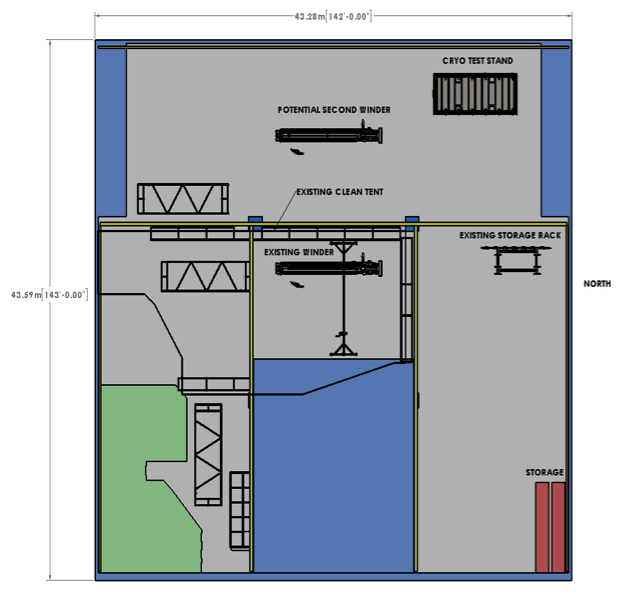
\includegraphics[height=0.28\textheight]{PSL-schematic.png} 
%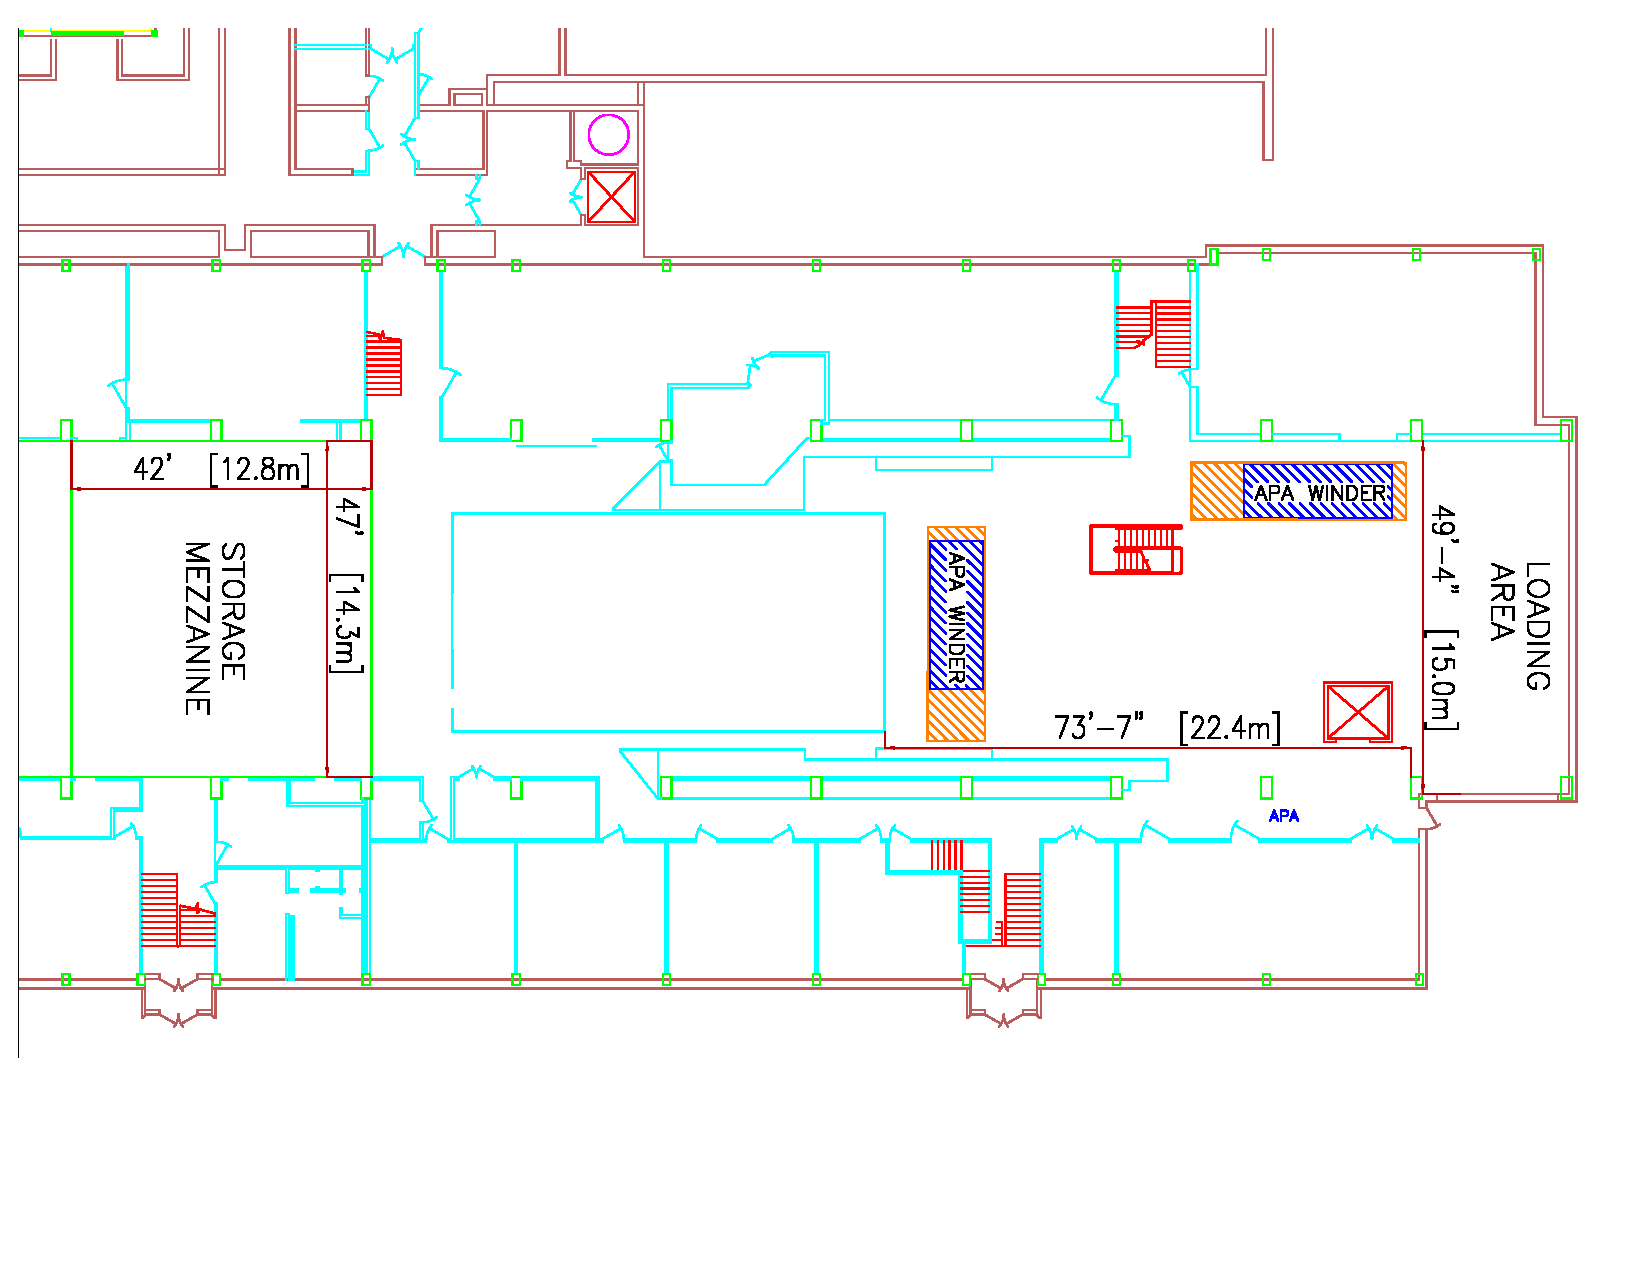
\includegraphics[height=0.26\textheight]{Chicago-2APA.pdf}
%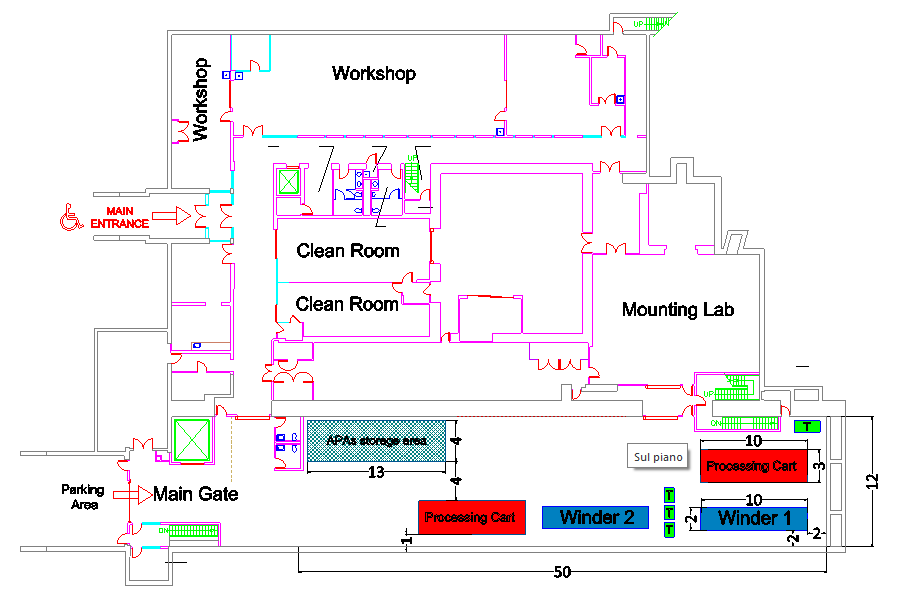
\includegraphics[height=0.27\textheight]{Yale-WL-2APA.png}
%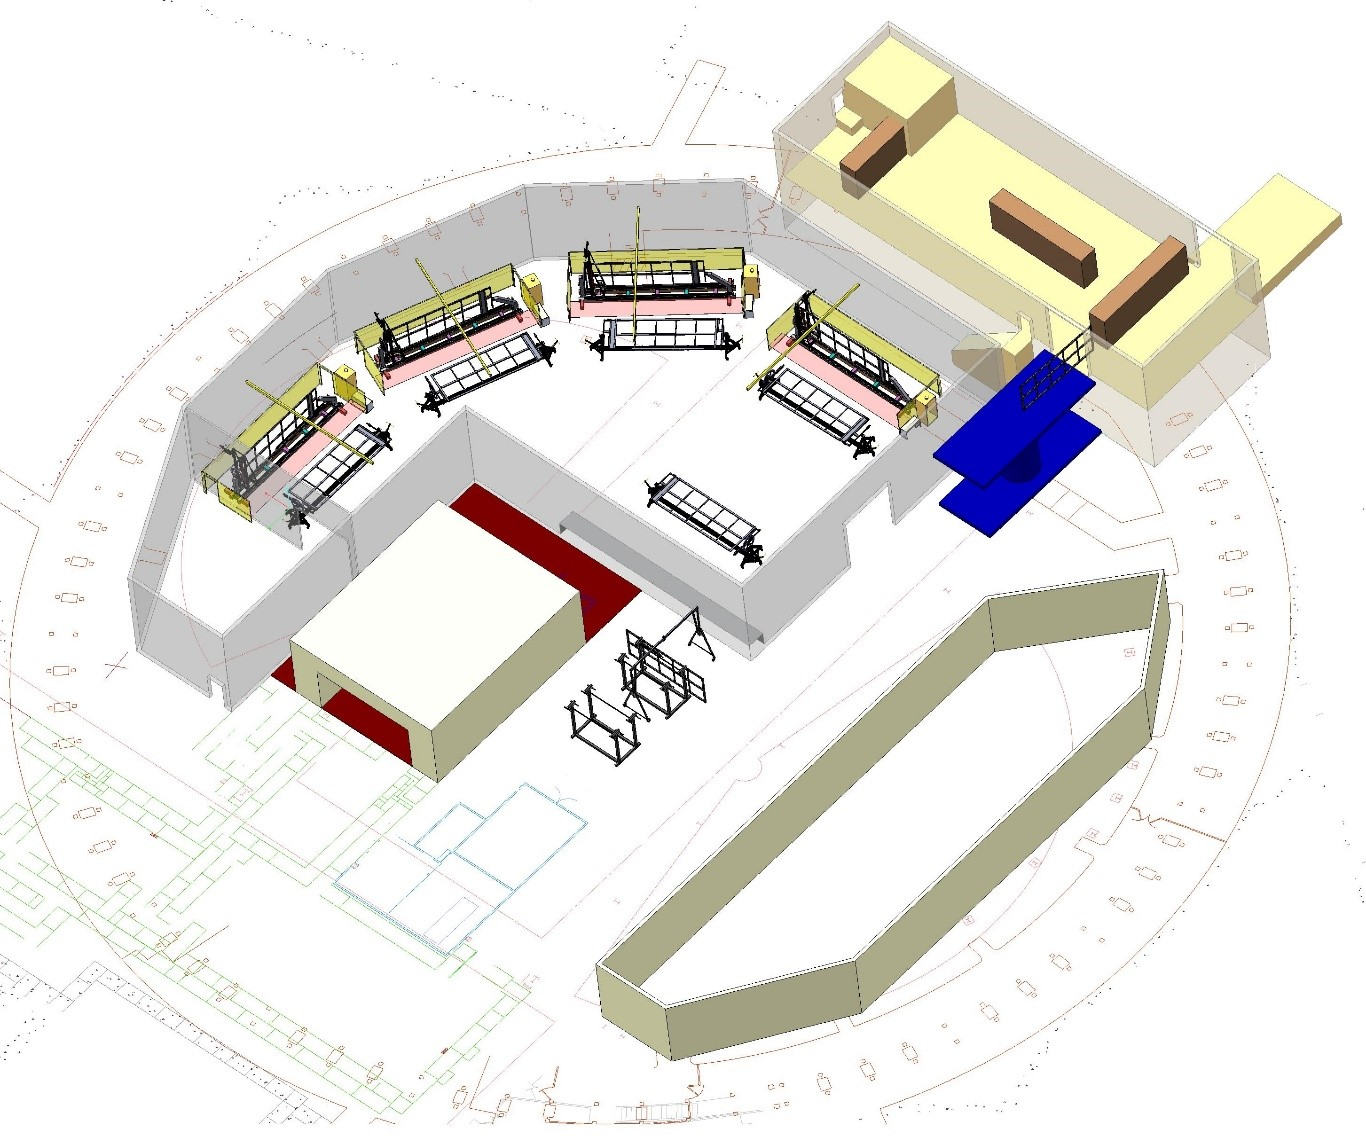
\includegraphics[height=0.27\textheight]{UK-production-factory-layout.jpg} 
%\end{dunefigure}

The University of Wisconsin has space available within the Physical Sciences Lab Rowe Technology Center. A portion of the facility has been used for the past two years for the ProtoDUNE project. There is approximately \SI{20000}{ft$^2$} (\SI{1850}{m$^2$}) available for DUNE and the possibility exists to expand the current clean tent to house another production line. 

ProtoDUNE construction has also taken place at Daresbury Lab.  The current facility cannot accommodate multiple production lines, but the ``Inner Hall'' on the Daresbury site has been identified as an area that is sufficiently large to be used for DUNE APA construction. It has good access and crane coverage throughout. Daresbury Laboratory management have agreed that the area is available, but investment is needed to establish a safe working environment. Preparation work for the construction area is underway to clear the current area of existing facilities, obsolete cranes, and ancillary equipment. Also planned is the renovation of a plant room which will be used for storage and as a shipping area. This work is ongoing. The production factory is being designed to hold 4 winding machines and associated process equipment and tooling. 

The Enrico Fermi Institute at the University of Chicago and the Wright Laboratory at Yale University each have the needed infrastructure to house up to two APA production lines. Development work that is relevant for local planning at each site has begun at those institutions as well.


%%%%%%%%%%%%%%%%%%%%%%%%%%%%%%%%%%%
\subsection{Assembly Procedures and Tooling}
\label{sec:fdsp-apa-assy}

\begin{comment}
A subset of procedures describing how to perform the step-by-step assembly of an APA was originally created prior to the finalization of the ProtoDUNE APA series of drawings, and assigned drawing numbers. During subsequent assemblies, these instructions have evolved due to the addition of better tooling, fixtures, jigs and more complete drawing documents.  The process steps contained in each procedure have also been changed to create a better match with the B.O.M. (Bill Of Materials) contained on each finalized drawing level.  Table~\ref{tab:assembly-docs} lists what documents are available related to each assembly level.  Currently these documents are being revised to reflect the latest evolution of these procedures that were used to assemble US-APA-4 for ProtoDUNE.

\begin{dunetable}[APA assembly documents]{lcc}{tab:assembly-docs}{Procedure documents for APA assembly.}   
APA Assembly Level & \textbf{Drawing No.} & \textbf{Assembly Instructions Doc.} \\ \toprowrule
APA Frame Assembly & 8757 004 & 8752Doc001 \\ 
                   &          & 8752Doc002 \\ \colhline
Comb Base and Mesh & 8757 003 & 8752Doc003 \\
				   &          & 8752Doc004 \\ \colhline
Four Wire Layers   & 8757 002 & ~~~~~8752Doc005 (X) \\
                   &          & ~~~~~8752Doc006 (V) \\
                   &          & ~~~~~8752Doc007 (U) \\
                   &          & ~~~~~8752Doc008 (G) \\ \colhline
Factory APA        & 8757 030 & 8752Doc009 \\
                   &          & 8752Doc010 \\ \colhline
Crating for Shipment & being finalized & being finalized \\
\end{dunetable}
\end{comment}

The central piece of equipment used in APA production is the custom-designed wire winder machine, shown in use in Figure~\ref{fig:winder-photos}.  An important centerpiece of the winder machine is the wiring head.  The head releases wire as motors move it up and down and across the frame, controlling the tension in the wire as it gets laid. Currently, the head then positions the wire at solder connection points for soldering by hand. The fully automated motion of the winder head is controlled by software, which is written in the widely used numerical control G programming language.  The winder also includes a built-in vision system to assist operators during winding, which is currently used at winding start-up to find a locator pin on the wire boards.  In the current scheme used for ProtoDUNE, during the winding process an APA moves on and off the winder machine multiple times for wiring, soldering, testing, etc.  

\begin{dunefigure}[Photos of the APA wire winding machine]{fig:winder-photos}
{Left: Partially wired ProtoDUNE APA on the winding machine at Daresbury Lab, UK. Right: Partially wired ProtoDUNE APA on the winding machine during wire tension measurements at University of Wisconsin, PSL.}
\setlength{\fboxsep}{0pt}
\setlength{\fboxrule}{0.5pt}
\fbox{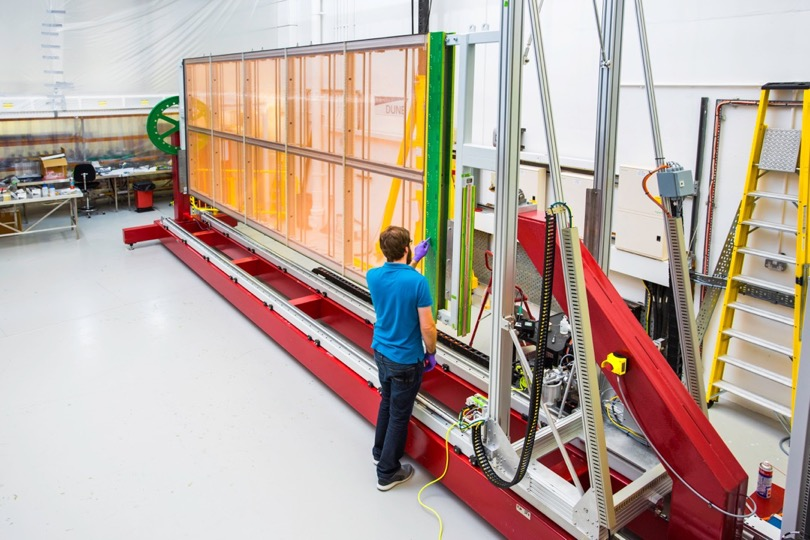
\includegraphics[height=0.3\textheight,trim=25mm 0mm 4mm 0mm,clip]{apa-on-winder-daresbury.jpg}}
\fbox{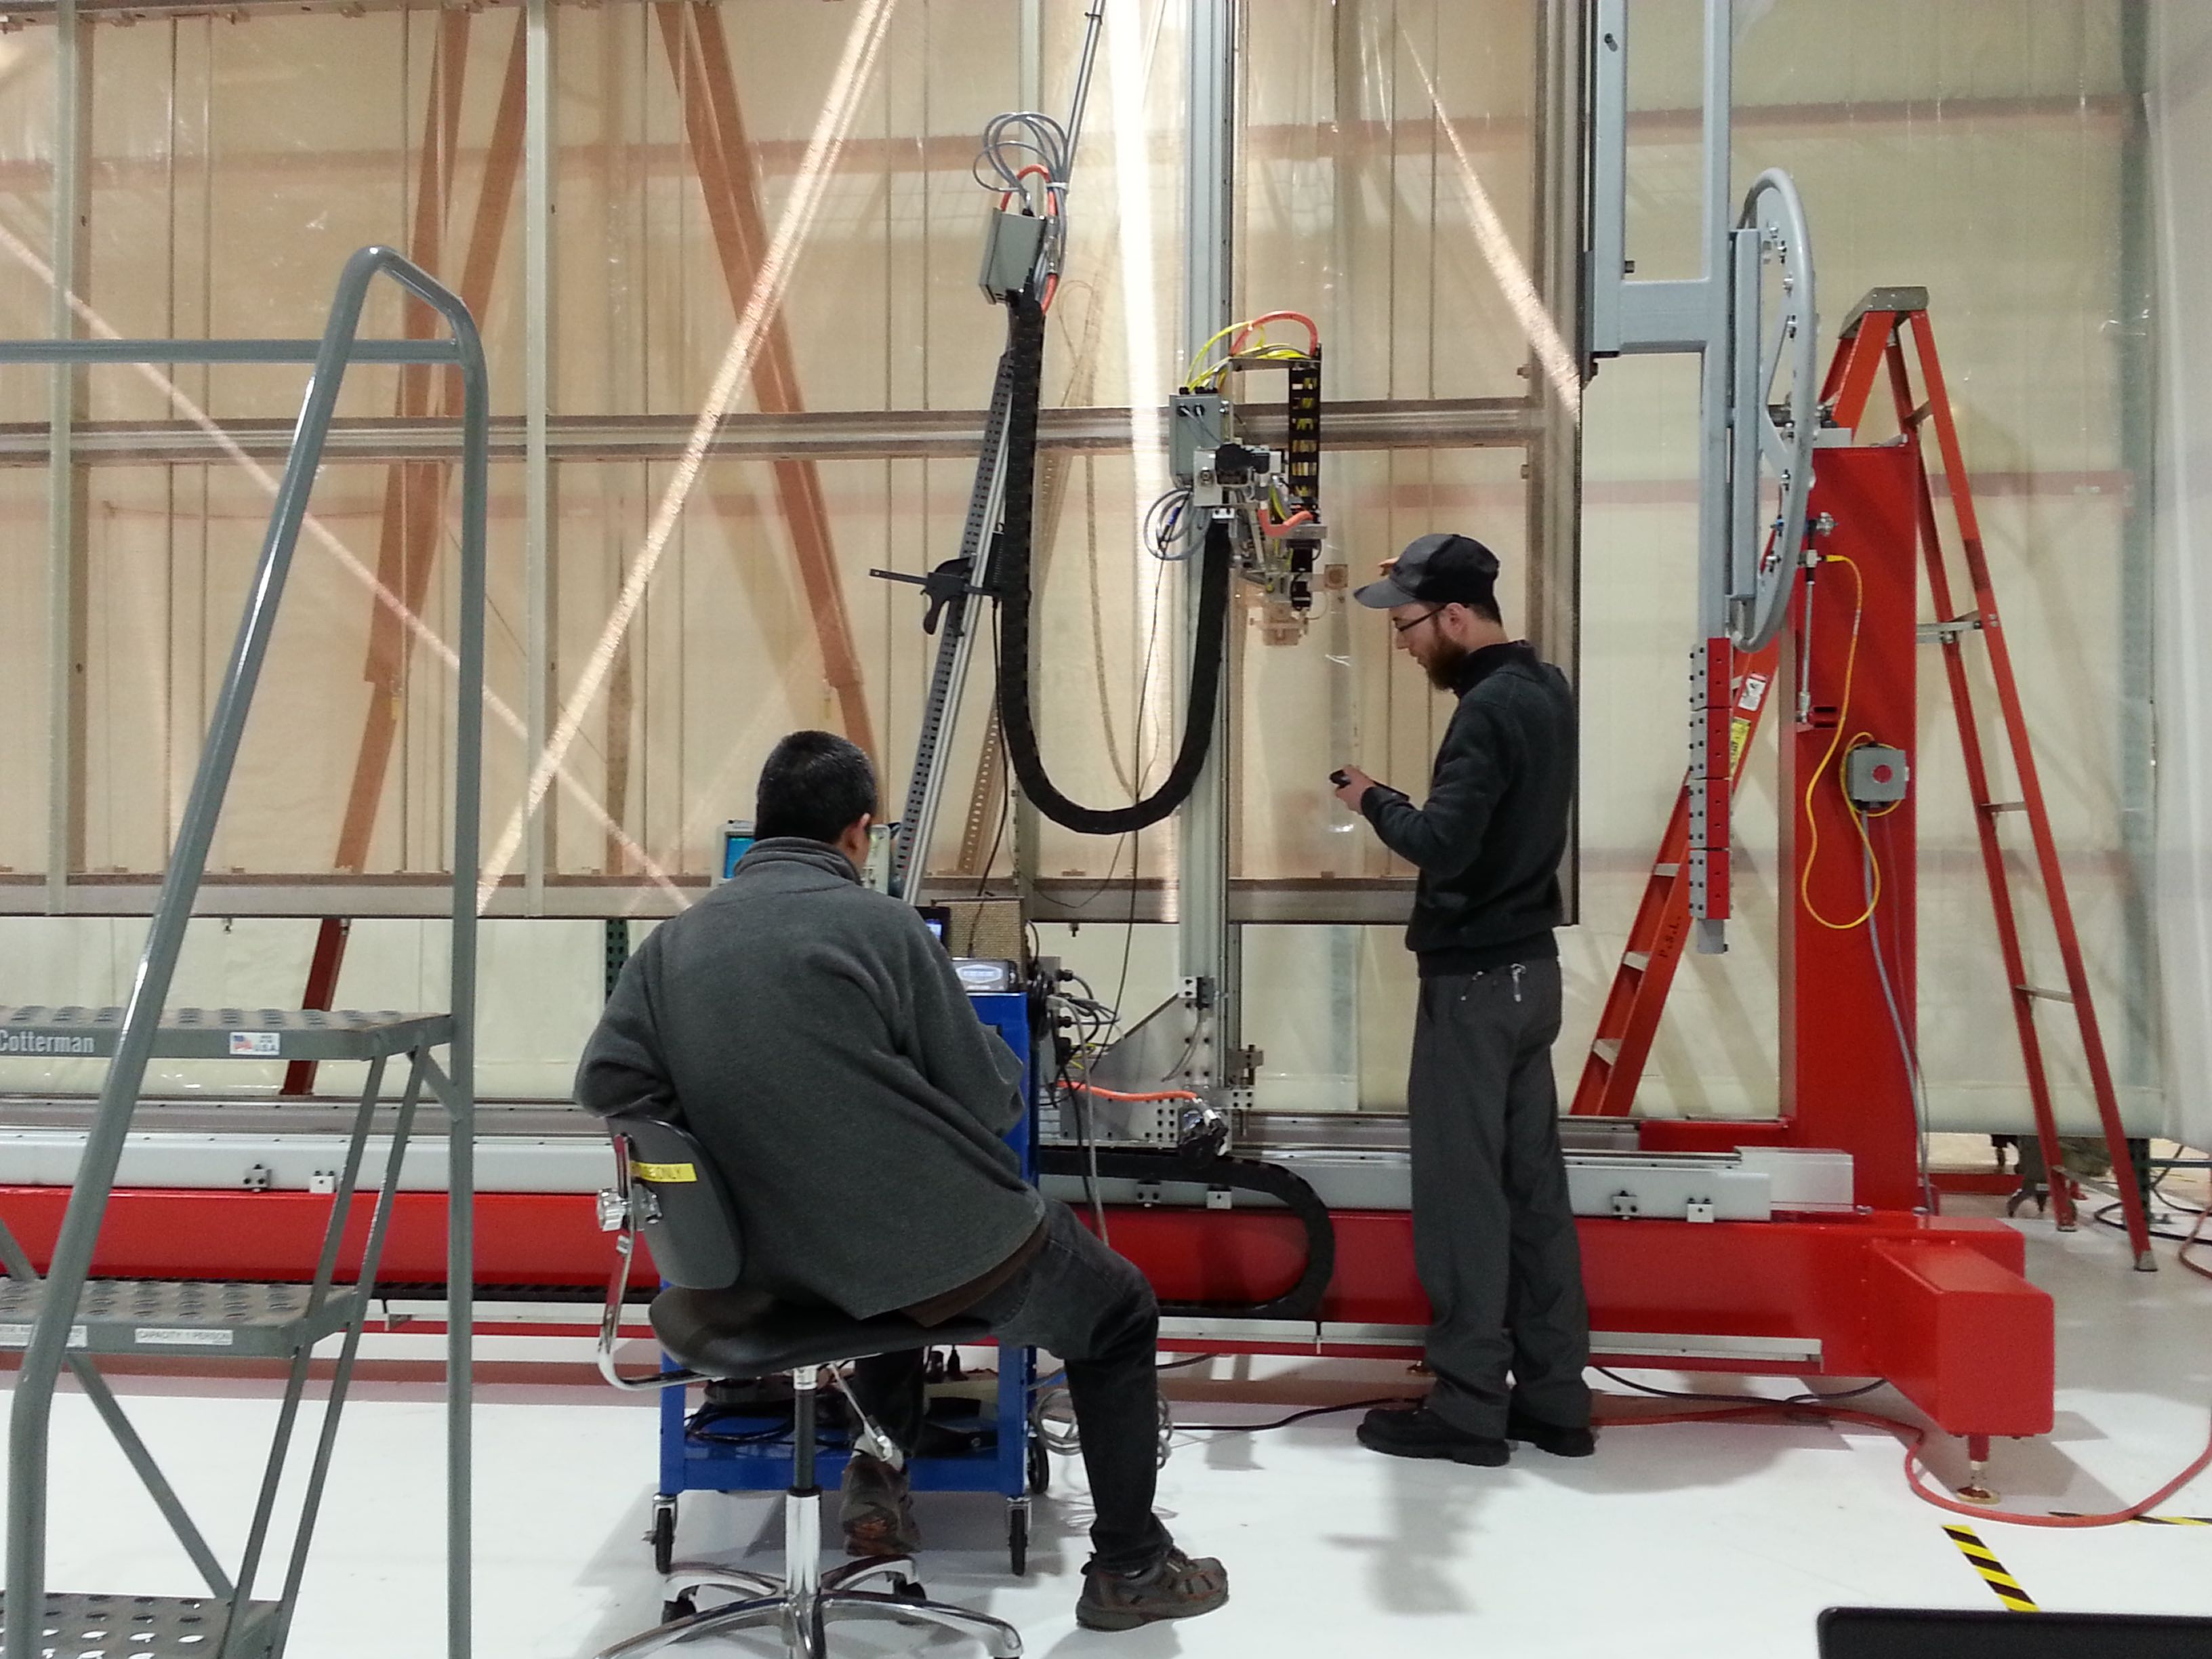
\includegraphics[height=0.3\textheight,trim=200mm 0mm 30mm 0mm,clip]{apa-tension-testing-psl.jpg}}
\end{dunefigure}

Two large process carts, shown in Figure~\ref{fig:apa-process-cart}, are used to move APAs around the assembly facility. 
%and also move them to a shipping/packing location area for loading into specialized crate containers. 
One process cart with regular casters remains in the assembly area and is maintained at a particular height that coordinates with other construction tooling such as jack stands and platform ladders. A second process cart has been fitted with specialized 360$^\circ$ rotating casters that allow the process cart loaded with a fully assembled APA to maneuver corners during the journey from the assembly area to the shipping/packing location.

Before wiring can begin, the first operation with a bare frame is to install the grounding mesh. In the ProtoDUNE design, a large jig is needed to hold the mesh in place for gluing. Once the jig is leveled sufficiently to the frame, a mesh sheet is laid into place and hold down bars are iteratively moved and repositioned until the mesh is flat and tight.  The outside edge of the mesh panel then gets epoxied, and the jig and hold down bars remain in place for a 12 hour epoxy cure cycle.  This process is then repeated for the next three shifts until all four panels of mesh have been attached to the bare APA frame.  As described below, changes to this lengthy procedure are being considered for DUNE APAs.  

Another custom construction jig is needed for installing the wire combs that hold the wires at intermediate points above the four cross beams of the APA.  Currently there are two jigs that can be loaded and installed at a time, and each installation requires a 6 hour epoxy cure cycle. %the two jigs are removed from the initial locations and placed in another two locations, on the same side of the APA.  Thus four comb bases are installed within one operation shift and the APA is left in this horizontal position to cure overnight.  The next day, the APA is flipped to the reverse side and the process is repeated for the other side. Figure~\ref{fig:apa-process-cart} shows the comb installation jig in use.  

\begin{dunefigure}[Photos of an APA on a process cart during construction]{fig:apa-process-cart}{(Left) APA being moved around a production facility on the process cart. (Right) APA frame with the grounding mesh already installed is shown sitting on a process cart.  Two technicians are using a custom jig to place the wire combs above a horizontal cross beam on the APA.}
\setlength{\fboxsep}{0pt}
\setlength{\fboxrule}{0.5pt}
\fbox{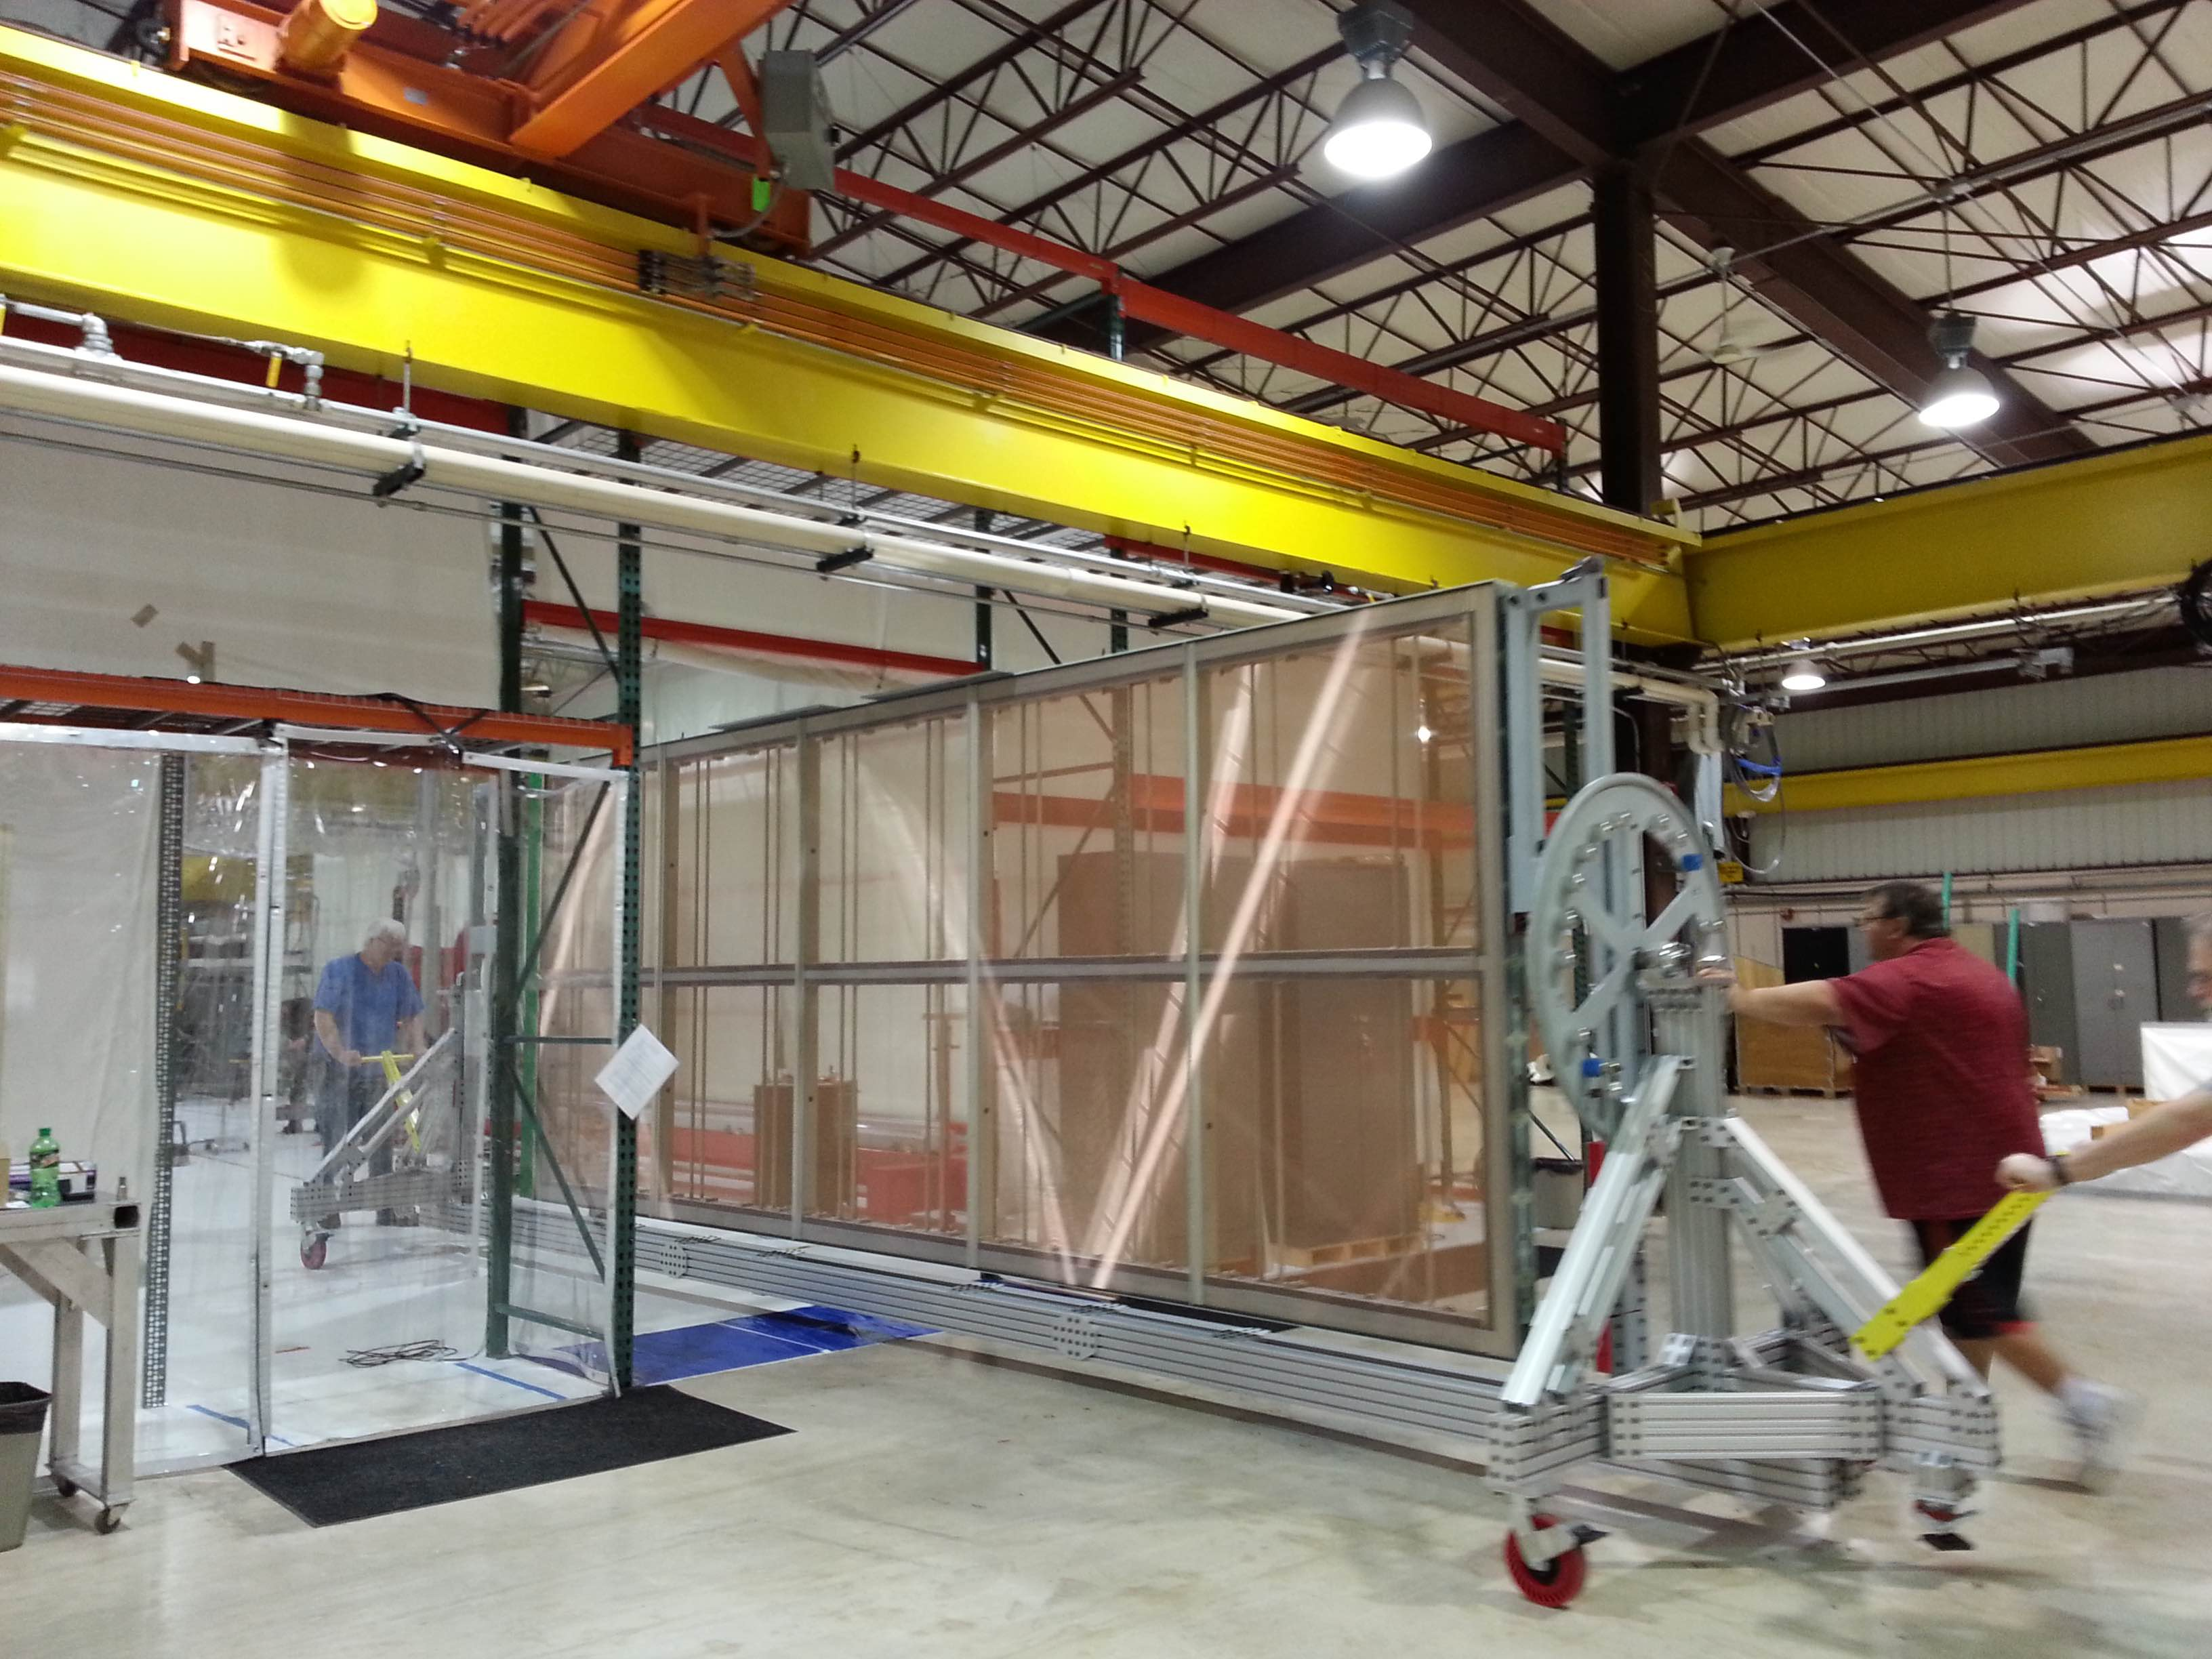
\includegraphics[height=0.24\textheight,trim=50mm 0mm 70mm 0mm,clip]{apa-process-cart.jpg}}
\fbox{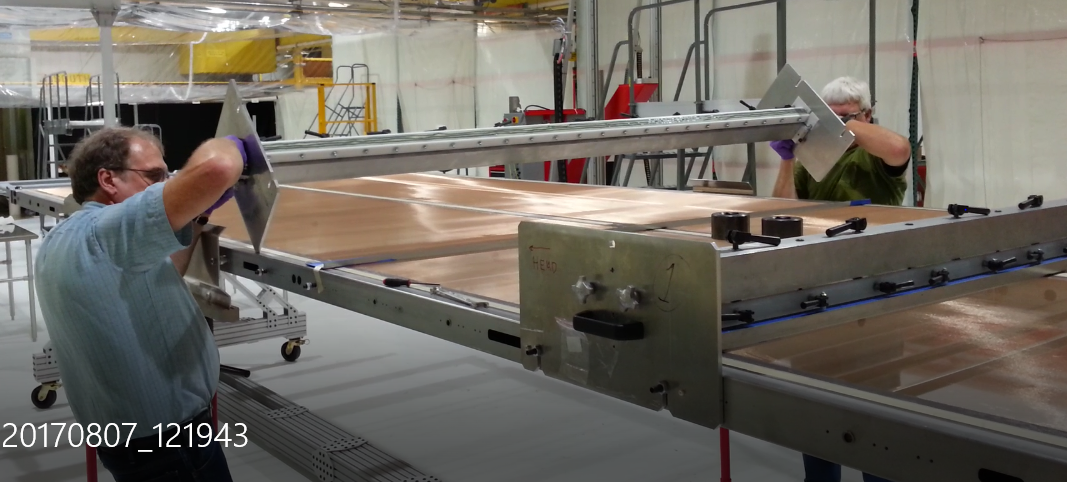
\includegraphics[height=0.24\textheight,trim=15mm 0mm 35mm 0mm,clip]{apa-comb-base-jig.png}}
\end{dunefigure}

%%%%%%%%%%%%%%%%%%%%%%%%%%%%%%%%%%%%%%%%%%%%%%%%%%%
\subsection{Material Supply}  

Ensuring the reliable supply of raw materials and parts to each of the factories is critical to keeping APA production on schedule through multiple years of construction. Here the consortium institutions will play a pivotal role taking on the responsibility for the delivery of APA sub-elements to each of the factories. Supplier institutions will have responsibility for the sourcing, inspection, cleaning, testing, quality assurance, and delivery of hardware to each of the factories. 

\begin{itemize}

\item Frame construction: We envision two sources of frames, one in the US and one in the UK. The institutions responsible will rely on many lessons learned from ProtoDUNE. The effort requires specialized resources and skills including a large assembly area, certified welding capability, large scale metrology tools and experience, and large scale tooling and crane support. Two approaches are under consideration for sourcing; one is a total outsource strategy with an industrial supplier, the other is to procure all of the major machined and welded components and then assemble and survey in-house. Material suppliers have been identified and used with good results on ProtoDUNE.

\item Mesh supply and construction: Elsewhere in this proposal we describe the current mesh installation procedure. However, our ProtoDUNE experience leads us to believe that moving to smaller self-supporting ``window screen'' panels will save assembly time and improve overall APA quality. An excellent source of mesh exists and was used on ProtoDUNE.

\item Wire procurement: Wire is a significant element in the assembly of an APA. There is approximately 24 km of wire wound on each unit. Through ProtoDUNE we have worked with an excellent supplier that has worked with us to provide wire that is of high quality and wound on spools that we provide. These spools are then used directly on the winder head with no additional handling or re-spooling required. Wire samples from each spool are strength tested prior to use.

\item Comb procurement: An institution will work with either our existing comb supplier or find additional suppliers that can meet our requirements. The ProtoDUNE supplier has been very reliable.

\item Wire wrapping board procurement: One or more consortium institutions will take on the responsibility of wire wrapping board supply. The side and foot boards are rather unique to suppliers as they have electrical traces and provide wire placement support through a separately bonded tooth strip. There are 276 boards per APA, or 41,400 needed for 150 APAs. The institutions that have responsibility for boards will spend time working with multiple vendors to reduce risk and ensure quality. 

\item Capacitor resistor boards: These boards are rather unique given their thickness, high voltage components, and leakage current requirements. A reliable source of bare boards was found for ProtoDUNE. Assembly and testing was performed at PSL. We will conduct a more exhaustive search of vendors that will be willing to take on assembly and test for the 3000 plus boards needed for DUNE.

\item Winders and tooling: We propose that PSL and Daresbury work together to supply tooling and winding machines for additional production lines at new locations and for additional lines in-house. This is a natural collaboration that has been in place for nearly two years on ProtoDUNE.

\end{itemize}


%%%%%%%%%%%%%%%%%%%%%%%%%%%%%%%%%%%%%%%%%%%%%%%%%%%%%%%%%%%
\subsection{Planned Improvements to Production Process}

Based on our ProtoDUNE experience, we have identified several potential improvements to tooling and process that will allow the APAs to be constructed in a more efficient and reliable manner, including:

\begin{itemize}

\item Wiring head design: Efforts to improve winder head performance are already underway. We envision improved tension control, continuous tension feedback, improved clutch, and an improvement to the compensator mechanism all leading to better, more consistent, and more reliable winder performance.  The current winding head uses a magnetic clutch mechanism that is manually adjusted to increase or decrease the tension of the wire as it is wound around the APA. The clutch regularly needs adjustment as the diameter of the wire on the spool reduces during the winding process. In addition, if the mechanism is run from a `cold start', it has been observed that the tension changes after $\sim$10 minutes of running. Experience winding the ProtoDUNE APAs has shown that it is difficult to maintain the target tension within tolerances (5$\pm$\SI{1}{N} for ProtoDUNE).

A solution to this issue is to design a winder head with active tension control. This can be achieved by replacing the magnetic clutch with a servo motor and introducing a potentiometer on a ``dancer arm'' for the feedback loop (see Figure~\ref{fig:winding-head}). This will only work if there are no signal losses when transferring the winding head to the compensator latching mechanism and back. The system can be driven in torque mode and will compensate for any wire spool changes and will be able to operate from a cold start. This development is well underway and tests are currently being carried out.

\begin{dunefigure}[Exploded view of the winding machine head]{fig:winding-head}
{Exploded view of winder head with active tension control.}
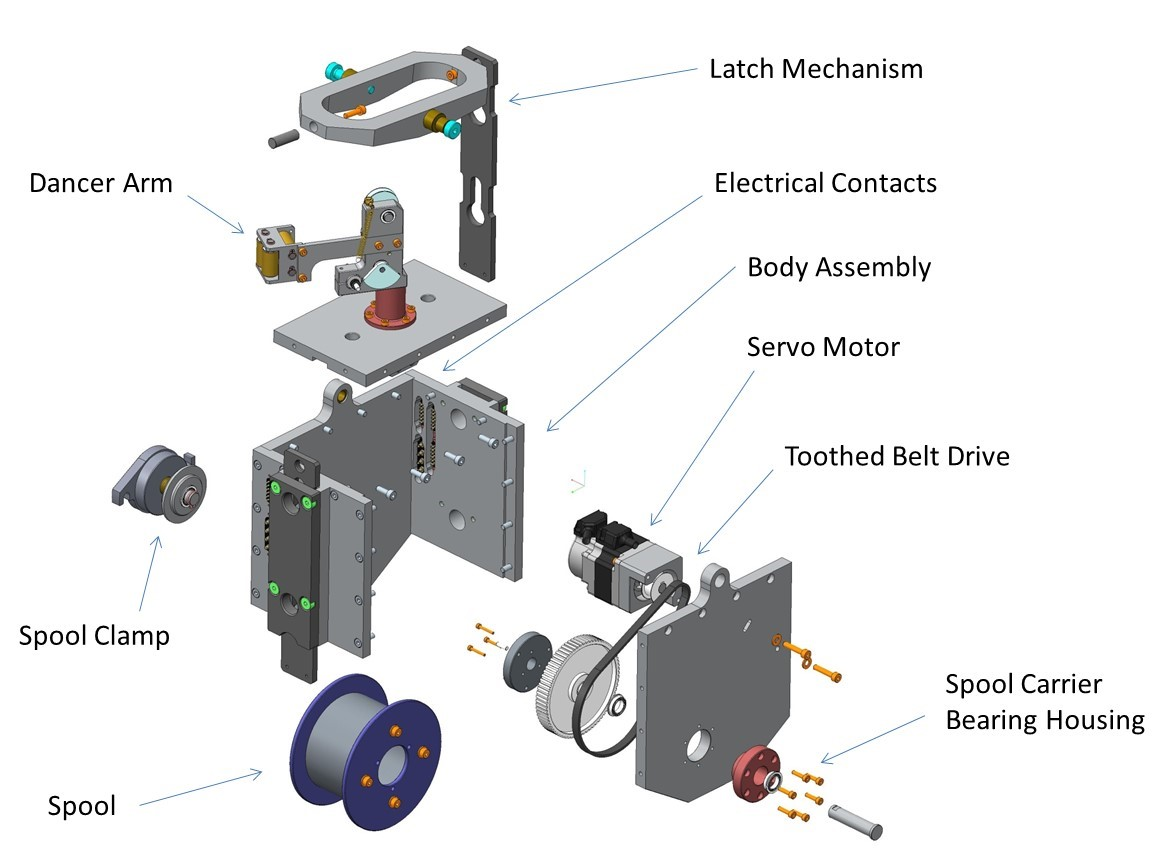
\includegraphics[width=0.7\textwidth]{apa-winder-head-with-active-tension-controls.jpg}
\end{dunefigure}

\item Winder interface arm design: The current winder interface only allows one-half of a wire plane to be wired at a time. The APA frame must be moved to the process cart where the interface arms are flipped 180$^\circ$ to wind the second half of the wire plane.  A new design concept, illustrated in Figure~\ref{fig:winding-dev}, will allow the winder head to pass from one side to the other in a nearly continuous fashion without removal from the winding machine.  The interface frames are replaced at either end by retractable linear guided shafts. These can be withdrawn to allow passing of the winding head around the frame over the full height of the frame. These shafts have conical ends and locate in shafts that are fixed to the internal frame tube to provide guided location. This design change does not alter the design of the frame. The design also allows for rotation in the winding machine, so that it should also be possible to carry out board installation and gluing \& soldering in the winding machine. This eliminates the need to transfer the APA to the process cart for the whole of the production operation, which is inherently a safer and faster production method as it cuts down the amount of handling of the APA.

\begin{dunefigure}[Winding machine schematic showing ongoing development]{fig:winding-dev}
{Work is ongoing to modify the wiring machine design to allow an APA frame to be rotated without removing it from the frame.  This would reduce the required handling of the frame during fabrication and speed production substantially.}
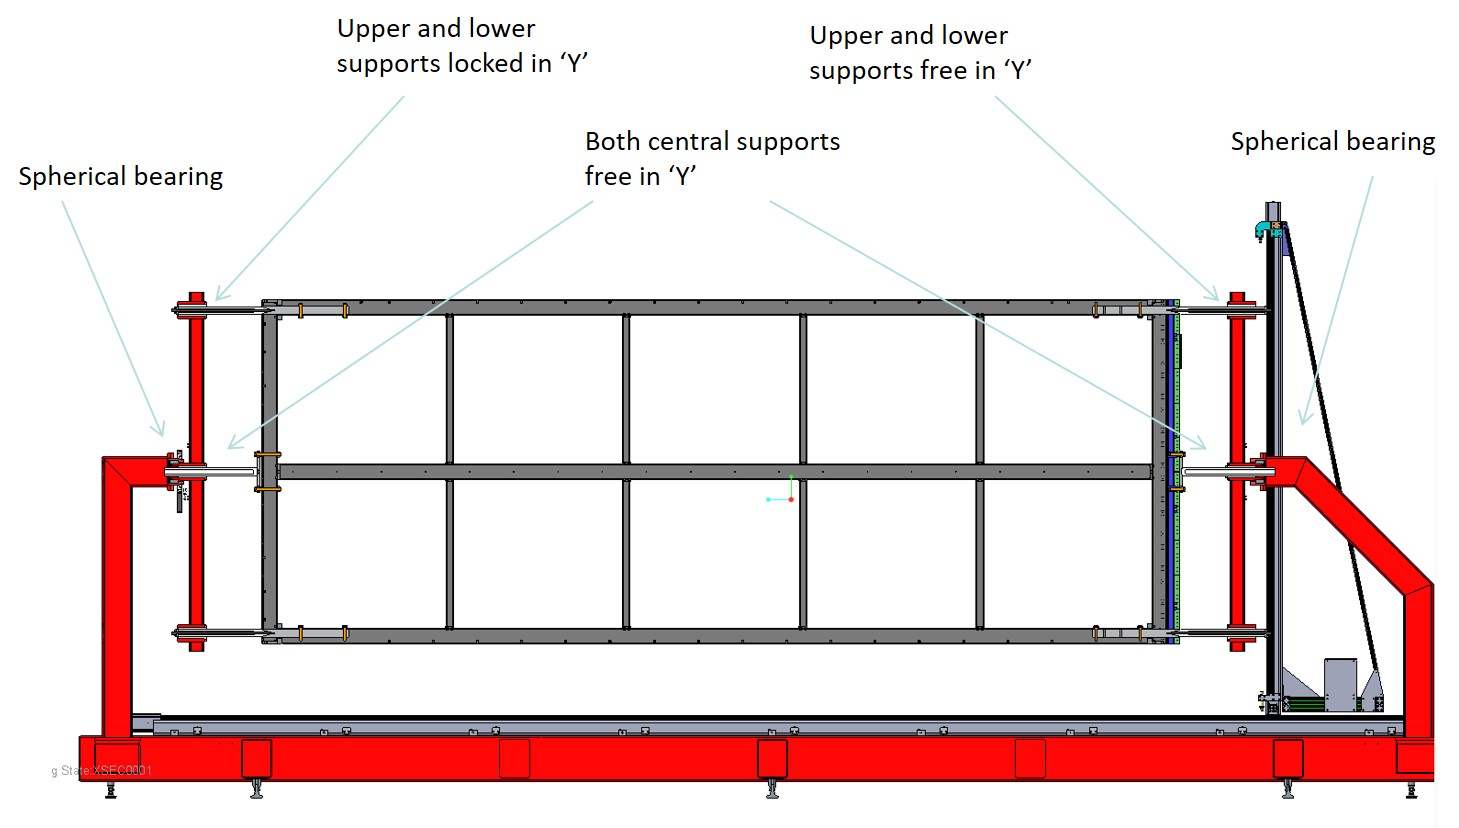
\includegraphics[width=0.95\textwidth]{apa-winding-machine-design-development.jpg} 
\end{dunefigure}

\item Modular mesh panels: The current approach to mesh installation is slow and cumbersome. We will improve this aspect of construction by moving toward a modular ``window screen'' design that will improve the reliability of the installed mesh (more uniform tension across the mesh), and allow much easier installation on the APA frame.

\item Epoxy process improvements: There are many epoxy application steps during the construction process. These steps require careful work that takes many hours between winding each successive wire plane. We already have concepts for improved epoxy application jigs from ProtoDUNE, and we will investigate whether epoxy pre-forms or accelerated heat curing can yield time or reliability improvements.

\item Automated soldering: Every solder joint on the 6 ProtoDUNE APAs was done by hand. We will investigate automated soldering techniques to improve process and reduce the amount of manual effort required. 

\item Wire tension measurement techniques: Verifying wire tension is an important, but time consuming process during construction. The current technique utilizes a laser photodiode tool mounted on the winder to measure tension one wire at a time. This takes many hours for each wire plane. Techniques are under development at the University of Manchester to electronically measure groups of 20 or more wires at one time. This technique will provide much faster tension measurements and shorter turnaround between wire planes. 

\item Winder maintenance plan: The approach to winder maintenance used during ProtoDUNE construction was not well formed. As a result, winding machine problems that can be traced back to lack of routine maintenance occurred from time-to-time, which shut the production line down until a repair or maintenance was performed. We will formulate a routine and preventive maintenance plan that should minimize winder downtime during DUNE APA production.
\end{itemize}


%%%%%%%%%%%%%%%%%%%%%%%%%%%%%%%%%%%%
\subsection{Quality Assurance and Quality Control in APA Production}
\label{sec:fdsp-apa-qa}

A key input to quality assurance for the DUNE APA design and manufacturing procedures is the experience with ProtoDUNE, including upcoming operations and data analysis results from the detector.  Much has already been learned regarding design, component testing, and fabrication procedures that will go into formulating the detailed design and plans for the DUNE APA construction project over the next year.  The set of final design drawings and detailed procedures documentation that will be generated over the next year leading to the TDR represent an important element of the quality assurance plan for the fabrication of the APAs.  

Summaries of all quality assurance testing performed for elements used in the final design of the APAs will also be prepared for the TDR.  Much data already exists, and again, ProtoDUNE will provide valuable additional information regarding the robustness of the detector components and construction.  

Below we discuss a few expected elements of a QA/QC plan for DUNE APA production.   

\subsubsection{Incoming Inspections}

Some components will require inspection and QC checks prior to use on an APA, including:

\begin{itemize}

\item Frame components: If the APA steel frames are produced in-house, then upon receipt of the rectangular hollow section steel for the frames, a selection procedure will be followed to choose the sections of the steel most suited to achieving the geometrical tolerances. 

\item Wire testing: The CuBe wire is provided on spools from the supplier. Samples from each spool will be strength tested prior to use on an APA.

\item Circuit boards: All circuit boards that get installed on an APA will be inspected for dimensional accuracy prior to being routed through various epoxy and cleaning processes as they are prepped for assembly. Inspection results will be documented, and if anomalies are found an electronic Non-Conformance report is written.  %Materials that can be re-worked to become conforming are set aside from inventory and re-worked.  If the material cannot be made usable, the material is kept in a non-conforming area sequestered from usable inventory.   

\item CR and $G$-plane bias board testing: Acceptance tests of these boards will include leakage current measurements ($<$\SI{0.5}{nA}) and continuity tests on each channel.  This test will be performed at room temperature. ProtoDUNE was used to perform design validation on over 100 boards that were cycled and tested at liquid nitrogen temperature. No failures were seen during these tests. 

\end{itemize}

\subsubsection{APA Acceptance Tests} 

The following are examples of quality control data that will be collected for each APA during production:  

\begin{itemize}

\item Frame flatness: A laser survey will be performed to measure the flatness of the assembled bare frame. Three sets of data are compiled into a map that shows the amount of bow, twist, and fold in the frame. Each of these parameters is compared to an allowable amount that will not cause wire plane-to-plane spacing to be out of tolerance ($\pm$\SI{0.5}{mm}).  A visual file will be created for each APA from measured data. A final frame survey will be completed after all electrical components have been installed, and the as-built plane-to-plane separations will be measured to verify the distance between adjacent wire planes.

\item Mesh to frame connection: To confirm sufficient electrical contact between these two components a resistance measurement will be taken in each of 20 zones of mesh bounded by the outside frame perimeter and the four cross beam ribs. This measurement will be completed immediately after mesh install, prior to any winding.

\item Wire tension: The tension of each wire will be measured after each new plane of wires is installed on an APA. The optimal target tension is still under discusion (was \SI{5}{N} in ProtoDUNE), as are teh necessary tolerances.  ProtoDUNE data, where the tensions have substantial variation, will provide important data for quantifying the impacts of varying tensions.  
%Wire tensions are required to be in the range 3.5--\SI{7.5}{N} for wires longer than \SI{750}{mm} and in the range 2.0--\SI{7.5}{N} for wires shorter than \SI{750}{mm}.

%\item Cleanliness: APAs are produced inside a class 100,000 clean area.  Particle counts are completed daily to verify cleanliness of the assembly area.  If counts are found outside of expected limits, measures are taken to re-clean the affected area and check with a follow-up particle count.
\end{itemize}


\subsubsection{Documentation} 

Each APA will have a ``Traveler'' document where specific assembly information is gathered, initially by hand on a paper copy, then entered into an electronic version for longer term storage.  The Traveler database will contain a detailed log of the production of each APA, including where and when the APA was built and the origin of all parts that were used in its construction. 

As assembly issues arise during the build of an APA, they will be gathered in an Issue Log for each APA and separate short reports will be created to provide details of what caused the occurrence, how the issue was immediately resolved, and what measures should be taken in the future to ensure the specific issue has a lower risk of occurring.  




